% Source-page vector redraw of the four function-graph options.
% Curves preserve visible topology only; coordinates are schematic.
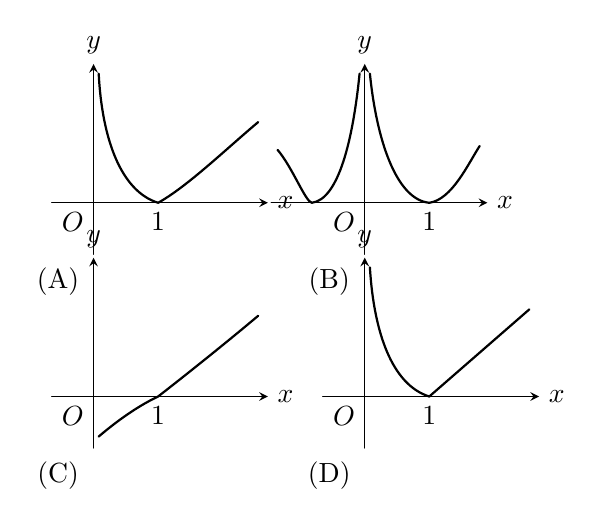
\begin{tikzpicture}[>=stealth, line cap=round, line join=round, scale=.82]
% Option A
\begin{scope}[shift={(0,0)}]
  \draw[->] (-.65,0)--(2.7,0) node[right] {$x$}; \draw[->] (0,-.8)--(0,2.15) node[above] {$y$};
  \node[below left] at (0,0) {$O$}; \node[below] at (1,0) {$1$}; \node at (-.55,-1.22) {(A)};
  \draw[thick] (.08,2.0) .. controls (.13,1.0) and (.42,.18) .. (1,0) .. controls (1.45,.25) and (2.05,.83) .. (2.55,1.25);
\end{scope}
% Option B
\begin{scope}[shift={(4.2,0)}]
  \draw[->] (-1.45,0)--(1.9,0) node[right] {$x$}; \draw[->] (0,-.8)--(0,2.15) node[above] {$y$};
  \node[below left] at (0,0) {$O$}; \node[below] at (1,0) {$1$}; \node at (-.55,-1.22) {(B)};
  \draw[thick] (-1.35,.82) .. controls (-1.12,.55) and (-.92,.02) .. (-.82,0) .. controls (-.4,.05) and (-.18,1.0) .. (-.08,2.0);
  \draw[thick] (.08,2.0) .. controls (.18,1.0) and (.48,.05) .. (1,0) .. controls (1.35,.05) and (1.6,.6) .. (1.78,.88);
\end{scope}
% Option C
\begin{scope}[shift={(0,-3.0)}]
  \draw[->] (-.65,0)--(2.7,0) node[right] {$x$}; \draw[->] (0,-.8)--(0,2.15) node[above] {$y$};
  \node[below left] at (0,0) {$O$}; \node[below] at (1,0) {$1$}; \node at (-.55,-1.22) {(C)};
  \draw[thick] (.08,-.62) .. controls (.28,-.45) and (.62,-.18) .. (1,0) .. controls (1.45,.35) and (2.05,.83) .. (2.55,1.25);
\end{scope}
% Option D
\begin{scope}[shift={(4.2,-3.0)}]
  \draw[->] (-.65,0)--(2.7,0) node[right] {$x$}; \draw[->] (0,-.8)--(0,2.15) node[above] {$y$};
  \node[below left] at (0,0) {$O$}; \node[below] at (1,0) {$1$}; \node at (-.55,-1.22) {(D)};
  \draw[thick] (.08,2.0) .. controls (.14,1.0) and (.42,.18) .. (1,0);
  \draw[thick] (1,0)--(2.55,1.35);
\end{scope}
\end{tikzpicture}
